% Source handout: :contentReference[oaicite:0]{index=0}
\documentclass[12pt]{article}

\usepackage[margin=1in]{geometry}
\usepackage{amsmath,amssymb,mathtools}
\usepackage{enumitem}
\usepackage{bm}
\usepackage{hyperref}
\usepackage{fancyhdr}
\usepackage{draftwatermark}
\usepackage{xcolor}
\usepackage{titlesec}
\usepackage{tikz}

%------------- TITLE AND METADATA -------------
\newcommand{\CourseCode}{MH1301 }
\newcommand{\CourseName}{Discrete Mathematics}
\newcommand{\DocType}{Tutorial 8}

\title{
\CourseCode \CourseName \\[0.3em]
\large \DocType
}
\author{
  Academic Year 2025/2026, Semester 2 \\[0.25em]
  \textit{Quantitative Research Society @NTU}
}
\date{\today}

%------------- HEADER & FOOTER (for page 2 onward) -------------
\fancypagestyle{main}{
  \fancyhf{}
  \fancyhead[L]{\CourseCode \CourseName}
  \fancyhead[R]{\href{https://qrsntu.org}{QRS@NTU}}
  \fancyfoot[C]{\thepage}
  \renewcommand{\headrulewidth}{0.4pt}
  \renewcommand{\footrulewidth}{0pt}
}

%------------- SIMPLE FOOTER (page 1 only) -------------
\fancypagestyle{plainfirst}{
  \fancyhf{}
  \renewcommand{\headrulewidth}{0pt}
  \renewcommand{\footrulewidth}{0pt}
  \fancyfoot[C]{\scriptsize\textcolor{gray}{\textit{For academic reference only. This document is provided for educational purposes and does not constitute an official question paper, answer key, or any formally authorised academic material. Its content is not guaranteed to be complete or accurate.}}}
}

%------------- WATERMARK -------------
\SetWatermarkText{Unofficial - QRS@NTU - qrsntu.org}
\SetWatermarkScale{1.0}
\SetWatermarkLightness{0.985}

%------------- SHORTCUTS -------------
\newcommand{\N}{\mathbb{N}}
\newcommand{\Z}{\mathbb{Z}}
\newcommand{\comp}[1]{\overline{#1}}

\setcounter{secnumdepth}{-1}
\setcounter{tocdepth}{3}

\begin{document}

\maketitle
\thispagestyle{plainfirst}
\pagestyle{main}

%====================================================
% OVERVIEW
%====================================================
\begin{center}
  \rule{0.82\textwidth}{0.4pt}\\[4pt]
  \textbf{Overview}\\[2pt]
  \rule{0.82\textwidth}{0.4pt}
\end{center}

\noindent
This tutorial develops the basic theory of graphs, with emphasis on:
\begin{itemize}[leftmargin=*]
  \item strong and weak connectivity in directed graphs;
  \item degree sequences and graph isomorphism;
  \item longest simple paths in connected graphs;
  \item Euler circuits and Euler trails;
  \item complements of graphs and self-complementary graphs;
  \item Hamilton circuits;
  \item edge bounds in terms of the number of connected components.
\end{itemize}

\noindent
\textbf{Question map.}
\begin{itemize}[leftmargin=*]
  \item Questions 1--3: connectivity, degree sequences, and longest paths.
  \item Questions 4--7: Euler circuits and one-stroke drawings.
  \item Question 8: Hamilton circuits in two displayed graphs.
  \item Question 9: upper and lower edge bounds for a graph with \(k\) connected components.
\end{itemize}

\newpage
%====================================================
% TABLE OF CONTENTS
%====================================================
\tableofcontents
\newpage

%====================================================
% QUESTION 1
%====================================================
\section{Question 1 (Strong and weak connectivity of directed graphs)}

\subsection{Problem}
Draw and determine whether each of these graphs is strongly connected and, if not, whether it is weakly connected.

\begin{enumerate}[label=(\alph*)]
\item \(G=(V,E)\) with \(V=\{a,b,c,d,e\}\), and directed edges
\[
E=\{(b,a),(b,c),(b,e),(e,a),(d,b),(c,d)\}.
\]

\item \(G=(V,E)\) with \(V=\{a,b,c,d,e\}\), and directed edges
\[
E=\{(a,d),(a,e),(b,a),(b,c),(d,b),(d,c),(e,b),(e,d)\}.
\]

\item \(G=(V,E)\) with \(V=\{a,b,c,d,e,f,g\}\), and directed edges
\[
E=\{(a,c),(a,g),(g,d),(d,c),(e,b),(b,f),(f,e)\}.
\]
\end{enumerate}

\subsection{Solution}

\subsubsection{Method 1: Direct reachability analysis}
\begin{enumerate}[label=(\alph*)]
\item The digraph is \emph{not} strongly connected. Indeed, the vertex \(a\) has out-degree \(0\), so there is no directed path from \(a\) to any other vertex. Therefore not every ordered pair of vertices is mutually reachable.

To decide weak connectivity, ignore edge directions. The resulting undirected graph has edges
\[
\{a,b\},\{b,c\},\{b,e\},\{a,e\},\{b,d\},\{c,d\},
\]
and every vertex is connected to \(b\) or to a vertex adjacent to \(b\). Thus the underlying undirected graph is connected.

Hence
\[
\boxed{\text{Graph (a) is not strongly connected, but it is weakly connected.}}
\]

\item This digraph is also \emph{not} strongly connected, because \(c\) has no outgoing edges. Hence there is no directed path from \(c\) to any other vertex, so strong connectivity fails.

Ignoring directions, the edges become
\[
\{a,d\},\{a,e\},\{a,b\},\{b,c\},\{b,d\},\{c,d\},\{b,e\},\{d,e\}.
\]
This undirected graph is connected: for example, \(c\) is adjacent to both \(b\) and \(d\), and the vertices \(a,b,d,e\) are all linked together.

Therefore
\[
\boxed{\text{Graph (b) is not strongly connected, but it is weakly connected.}}
\]

\item This digraph is \emph{not} strongly connected. In fact it is not even weakly connected.

Ignoring directions, the edges become
\[
\{a,c\},\{a,g\},\{g,d\},\{d,c\},\{e,b\},\{b,f\},\{f,e\}.
\]
So the underlying undirected graph has two connected components:
\[
\{a,c,d,g\}
\qquad\text{and}\qquad
\{b,e,f\}.
\]
Since the underlying undirected graph is disconnected, the digraph is not weakly connected; consequently it cannot be strongly connected either.

Hence
\[
\boxed{\text{Graph (c) is neither strongly connected nor weakly connected.}}
\]
\end{enumerate}

\subsubsection{Method 2: Strongly connected components and condensation}
\begin{enumerate}[label=(\alph*)]
\item In graph (a), the vertices \(b,c,d\) form a directed cycle
\[
b\to c\to d\to b,
\]
so \(\{b,c,d\}\) is one strongly connected component. The vertex \(e\) has a directed edge to \(a\), but there is no path back from \(a\) to \(e\), so \(e\) is its own strongly connected component. The vertex \(a\) is a sink, so \(\{a\}\) is another strongly connected component. Thus the strongly connected components are
\[
\{b,c,d\},\qquad \{e\},\qquad \{a\}.
\]
Since there is more than one strongly connected component, the graph is not strongly connected. But the condensation graph is connected as an undirected graph, so the original digraph is weakly connected.

Therefore
\[
\boxed{\text{(a) is not strongly connected, but is weakly connected.}}
\]

\item In graph (b), the vertices \(a,b,d,e\) lie in one strongly connected component:
\[
a\to d\to b\to a,\qquad a\to e\to b\to a,\qquad e\to d\to b\to a\to e,
\]
so every one of \(a,b,d,e\) can reach every other. The vertex \(c\) is a sink, so \(\{c\}\) is a separate strongly connected component. Hence the strongly connected components are
\[
\{a,b,d,e\},\qquad \{c\}.
\]
Thus the graph is not strongly connected. The condensation graph consists of one edge from the first component to \(\{c\}\), so its underlying undirected graph is connected. Hence the digraph is weakly connected.

Thus
\[
\boxed{\text{(b) is not strongly connected, but is weakly connected.}}
\]

\item In graph (c), the vertices \(e,b,f\) form a directed cycle
\[
e\to b\to f\to e,
\]
so \(\{e,b,f\}\) is one strongly connected component. In the other part of the graph, there are directed edges
\[
a\to g,\qquad g\to d,\qquad d\to c,\qquad a\to c,
\]
but no directed cycles, so each of \(a,g,d,c\) forms its own strongly connected component. Moreover, there is no edge at all between the set \(\{a,c,d,g\}\) and the set \(\{b,e,f\}\) in the underlying undirected graph. So the digraph is not weakly connected.

Hence
\[
\boxed{\text{(c) is neither strongly connected nor weakly connected.}}
\]
\end{enumerate}

\newpage

%====================================================
% QUESTION 2
%====================================================
\section{Question 2 (Degree sequences and isomorphism)}

\subsection{Problem}
The degree sequence of a graph \(G=(V,E)\) is the sequence of length \(n=|V|\) that contains \(\deg(v)\) for all \(v\in V\). Usually it is sorted non-decreasingly.

\begin{enumerate}[label=(\alph*)]
\item State the degree sequence of the following graphs:

\begin{center}
\begin{minipage}{0.42\textwidth}
\centering
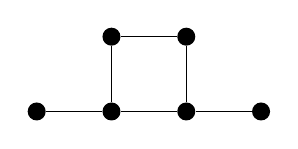
\begin{tikzpicture}[scale=0.95, every node/.style={circle, fill=black, inner sep=2.3pt}]
\node (a) at (0,0) {};
\node (b) at (1,0) {};
\node (c) at (2,0) {};
\node (d) at (3,0) {};
\node (e) at (1,1) {};
\node (f) at (2,1) {};
\draw (a)--(b)--(c)--(d);
\draw (b)--(e)--(f)--(c);
\end{tikzpicture}

\vspace{0.2em}
Graph 1
\end{minipage}
\hfill
\begin{minipage}{0.42\textwidth}
\centering
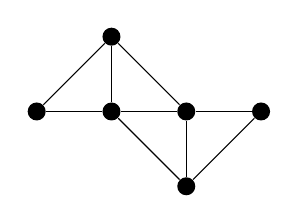
\begin{tikzpicture}[scale=0.95, every node/.style={circle, fill=black, inner sep=2.3pt}]
\node (l) at (0,0) {};
\node (m) at (1,0) {};
\node (u) at (1,1) {};
\node (n) at (2,0) {};
\node (r) at (3,0) {};
\node (d) at (2,-1) {};
\draw (l)--(m)--(n)--(r);
\draw (u)--(l);
\draw (u)--(m);
\draw (u)--(n);
\draw (m)--(d);
\draw (n)--(d);
\draw (r)--(d);
\end{tikzpicture}

\vspace{0.2em}
Graph 2
\end{minipage}
\end{center}

\item Prove that two graphs that do not have the same degree sequence cannot be isomorphic.
\end{enumerate}

\subsection{Solution}

\subsubsection{Method 1: Compute degrees directly and use degree preservation under isomorphism}
\begin{enumerate}[label=(\alph*)]
\item For Graph 1, the four bottom vertices have degrees
\[
1,\ 3,\ 3,\ 1
\]
from left to right, and the two top vertices each have degree \(2\). So the degree sequence, sorted non-decreasingly, is
\[
(1,1,2,2,3,3).
\]
Hence
\[
\boxed{\text{Graph 1 has degree sequence }(1,1,2,2,3,3).}
\]

For Graph 2, the leftmost and rightmost vertices each have degree \(2\), the top and bottom central vertices each have degree \(3\), and the two middle horizontal vertices each have degree \(4\). So the degree sequence is
\[
(2,2,3,3,4,4).
\]
Thus
\[
\boxed{\text{Graph 2 has degree sequence }(2,2,3,3,4,4).}
\]

\newpage
\item Let \(G\) and \(H\) be isomorphic graphs, and let
\[
f:V(G)\to V(H)
\]
be an isomorphism. By definition, \(f\) is a bijection preserving adjacency:
\[
uv\in E(G)\iff f(u)f(v)\in E(H).
\]
Fix a vertex \(u\in V(G)\). The neighbors of \(u\) in \(G\) are carried bijectively by \(f\) onto the neighbors of \(f(u)\) in \(H\). Hence
\[
\deg_G(u)=\deg_H(f(u)).
\]
Since \(f\) is a bijection on the vertices, the multiset of vertex degrees of \(G\) is exactly the same as the multiset of vertex degrees of \(H\). Therefore, after sorting, the degree sequences must be identical.

Consequently, if two graphs do \emph{not} have the same degree sequence, they cannot be isomorphic. Hence
\[
\boxed{\text{Different degree sequences imply the graphs are not isomorphic.}}
\]
\end{enumerate}

\subsubsection{Method 2: Adjacency-matrix row sums}
\begin{enumerate}[label=(\alph*)]
\item The degree sequences are the same as in Method 1:
\[
\boxed{(1,1,2,2,3,3)\ \text{for Graph 1},\qquad (2,2,3,3,4,4)\ \text{for Graph 2}.}
\]

\item Let \(A_G\) be the adjacency matrix of \(G\), and \(A_H\) the adjacency matrix of \(H\). If \(G\cong H\), then there exists a permutation matrix \(P\) such that
\[
A_H=P^{T}A_G P.
\]
The degree of a vertex is the sum of the entries in the corresponding row of the adjacency matrix. Multiplying by a permutation matrix on the left and right merely reorders the rows and columns, so the list of row sums of \(A_H\) is just a permutation of the list of row sums of \(A_G\).

Therefore isomorphic graphs must have the same multiset of degrees, and hence the same sorted degree sequence. So if two graphs have different degree sequences, they cannot be isomorphic.

Thus
\[
\boxed{\text{If the degree sequences differ, the graphs are not isomorphic.}}
\]
\end{enumerate}

\newpage

%====================================================
% QUESTION 3
%====================================================
\section{Question 3 (Longest simple paths in a connected graph)}

\subsection{Problem}
If a graph \(G\) is connected and has no simple path with length greater than \(k\), prove that every two simple paths in \(G\) of length \(k\) have at least one vertex in common.

\subsection{Solution}

\subsubsection{Method 1: Shortest-Connector Contradiction}

Let
\[
P=u_0u_1\cdots u_k,
\qquad
Q=v_0v_1\cdots v_k
\]
be two simple paths of length \(k\). We prove that
\[
V(P)\cap V(Q)\neq \varnothing.
\]

Suppose, for contradiction, that
\[
V(P)\cap V(Q)=\varnothing.
\]
Since \(G\) is connected, there exists a path joining a vertex of \(P\) to a vertex of \(Q\). Among all such paths, choose one of minimum length:
\[
R=x_0x_1\cdots x_t,
\]
where
\[
x_0=u_i\in V(P),
\qquad
x_t=v_j\in V(Q).
\]
Since \(P\) and \(Q\) are vertex-disjoint,
\[
t\ge 1.
\]

We claim that
\[
\{x_1,\dots,x_{t-1}\}\cap \bigl(V(P)\cup V(Q)\bigr)=\varnothing.
\]
Indeed, if \(x_s\in V(P)\) for some \(1\le s\le t-1\), then
\[
x_sx_{s+1}\cdots x_t
\]
is a shorter path from \(P\) to \(Q\), contradiction. Similarly, if \(x_s\in V(Q)\), then
\[
x_0x_1\cdots x_s
\]
is a shorter path from \(P\) to \(Q\), contradiction.

Now \(u_i\) divides \(P\) into two subpaths of lengths
\[
i
\qquad\text{and}\qquad
k-i.
\]
Therefore
\[
\max\{i,k-i\}\ge \left\lceil \frac{k}{2}\right\rceil.
\]
Choose the longer subpath of \(P\) from \(u_i\) to one endpoint of \(P\), and denote it by \(P'\). Then
\[
\ell(P')\ge \left\lceil \frac{k}{2}\right\rceil.
\]

Similarly, \(v_j\) divides \(Q\) into two subpaths of lengths
\[
j
\qquad\text{and}\qquad
k-j,
\]
so the longer subpath \(Q'\) from \(v_j\) to one endpoint of \(Q\) satisfies
\[
\ell(Q')\ge \left\lceil \frac{k}{2}\right\rceil.
\]

Since \(P\) and \(Q\) are vertex-disjoint and the internal vertices of \(R\) avoid \(P\cup Q\), the concatenation
\[
P' \cup R \cup Q'
\]
is a simple path. Its length is at least
\[
\ell(P')+\ell(R)+\ell(Q')
\ge
\left\lceil \frac{k}{2}\right\rceil
+t+
\left\lceil \frac{k}{2}\right\rceil.
\]
Since \(t\ge 1\),
\[
\ell(P'\cup R\cup Q')
\ge
2\left\lceil \frac{k}{2}\right\rceil+1
>k.
\]
This contradicts the hypothesis that \(G\) has no simple path of length greater than \(k\).

Hence
\[
V(P)\cap V(Q)\neq \varnothing.
\]
Therefore
\[
\boxed{\text{Every two simple paths of length }k\text{ in }G\text{ have at least one common vertex.}}
\]

\newpage
\subsubsection{Method 2: Longest-Path Intersection Theorem}

We use the following theorem.

\medskip
\noindent
\textbf{Theorem.}
In a connected graph, any two longest simple paths have a common vertex.

\medskip
\noindent
\textbf{Proof.}
Let
\[
P=u_0u_1\cdots u_m,
\qquad
Q=v_0v_1\cdots v_m
\]
be two longest simple paths in a connected graph \(G\). Suppose
\[
V(P)\cap V(Q)=\varnothing.
\]
Since \(G\) is connected, choose a shortest path
\[
R=x_0x_1\cdots x_t
\]
from \(P\) to \(Q\), where
\[
x_0=u_i\in V(P),
\qquad
x_t=v_j\in V(Q).
\]
Then \(t\ge 1\), and by the minimality of \(R\),
\[
\{x_1,\dots,x_{t-1}\}\cap \bigl(V(P)\cup V(Q)\bigr)=\varnothing.
\]

From \(u_i\), choose the longer subpath of \(P\) to an endpoint. Its length is
\[
\max\{i,m-i\}\ge \left\lceil \frac{m}{2}\right\rceil.
\]
From \(v_j\), choose the longer subpath of \(Q\) to an endpoint. Its length is
\[
\max\{j,m-j\}\ge \left\lceil \frac{m}{2}\right\rceil.
\]
Together with \(R\), these two subpaths form a simple path of length at least
\[
\left\lceil \frac{m}{2}\right\rceil
+1+
\left\lceil \frac{m}{2}\right\rceil
>m.
\]
This contradicts the maximality of \(P\) and \(Q\). Therefore
\[
V(P)\cap V(Q)\neq \varnothing.
\]
This proves the theorem.
\[
\Box
\]

Now return to the given problem. Since \(G\) has no simple path of length greater than \(k\), every simple path of length \(k\) is a longest simple path. Hence, by the theorem, any two simple paths of length \(k\) have a common vertex.

Therefore
\[
\boxed{\text{Every two simple paths of length }k\text{ in }G\text{ have at least one common vertex.}}
\]

\newpage
\subsubsection{Method 3: Contrapositive Path-Attachment Lemma}

We prove the contrapositive.

The desired statement is
\[
\left(
\text{no simple path has length greater than }k
\right)
\Longrightarrow
\left(
\text{any two length-}k\text{ simple paths intersect}
\right).
\]
Its contrapositive is
\[
\left(
\exists \text{ two vertex-disjoint simple paths of length }k
\right)
\Longrightarrow
\left(
\exists \text{ a simple path of length greater than }k
\right).
\]

Assume that there exist two vertex-disjoint simple paths
\[
P=u_0u_1\cdots u_k,
\qquad
Q=v_0v_1\cdots v_k.
\]
Since \(G\) is connected, choose a shortest connector
\[
R=x_0x_1\cdots x_t,
\]
where
\[
x_0=u_i\in V(P),
\qquad
x_t=v_j\in V(Q).
\]
Then
\[
t\ge 1
\]
and, by minimality,
\[
\{x_1,\dots,x_{t-1}\}\cap \bigl(V(P)\cup V(Q)\bigr)=\varnothing.
\]

Define
\[
\alpha=\max\{i,k-i\},
\qquad
\beta=\max\{j,k-j\}.
\]
Then
\[
\alpha\ge \left\lceil \frac{k}{2}\right\rceil,
\qquad
\beta\ge \left\lceil \frac{k}{2}\right\rceil.
\]
Take the length-\(\alpha\) subpath of \(P\) from \(u_i\) to an endpoint of \(P\), the connector \(R\), and the length-\(\beta\) subpath of \(Q\) from \(v_j\) to an endpoint of \(Q\). Their concatenation is a simple path of length
\[
\alpha+t+\beta.
\]
Thus
\[
\alpha+t+\beta
\ge
\left\lceil \frac{k}{2}\right\rceil
+1+
\left\lceil \frac{k}{2}\right\rceil
>k.
\]
Hence \(G\) contains a simple path of length greater than \(k\).

Therefore, by contrapositive, if \(G\) has no simple path of length greater than \(k\), then no two length-\(k\) simple paths can be vertex-disjoint. Hence every two simple paths of length \(k\) have a common vertex.

\[
\boxed{\text{Every two simple paths of length }k\text{ in }G\text{ have at least one common vertex.}}
\]

\subsubsection{Method 4: Extremal Separation Principle}

Let
\[
\mathcal{P}_k=\{P:\ P\text{ is a simple path of length }k\}.
\]
The hypothesis implies that every \(P\in \mathcal{P}_k\) is extremal, i.e. longest possible.

Suppose there exist
\[
P=u_0u_1\cdots u_k,
\qquad
Q=v_0v_1\cdots v_k
\]
such that
\[
V(P)\cap V(Q)=\varnothing.
\]
Because \(G\) is connected,
\[
d(V(P),V(Q))<\infty.
\]
Choose \(u_i\in V(P)\) and \(v_j\in V(Q)\) such that
\[
d(u_i,v_j)=d(V(P),V(Q)).
\]
Let
\[
R
\]
be a shortest \(u_i\)-\(v_j\) path. Then \(R\) meets \(P\cup Q\) only at its endpoints; otherwise \(d(V(P),V(Q))\) would be smaller.

Now
\[
\max\{d_P(u_i,u_0),d_P(u_i,u_k)\}
=
\max\{i,k-i\}
\ge
\left\lceil\frac{k}{2}\right\rceil,
\]
and
\[
\max\{d_Q(v_j,v_0),d_Q(v_j,v_k)\}
=
\max\{j,k-j\}
\ge
\left\lceil\frac{k}{2}\right\rceil.
\]
Thus there exist endpoints \(u_r\in\{u_0,u_k\}\) and \(v_s\in\{v_0,v_k\}\) such that
\[
d_P(u_i,u_r)\ge \left\lceil\frac{k}{2}\right\rceil,
\qquad
d_Q(v_j,v_s)\ge \left\lceil\frac{k}{2}\right\rceil.
\]
Therefore
\[
u_r \leadsto_P u_i \leadsto_R v_j \leadsto_Q v_s
\]
is a simple path of length at least
\[
\left\lceil\frac{k}{2}\right\rceil
+
1
+
\left\lceil\frac{k}{2}\right\rceil
>k,
\]
contradicting extremality.

Hence
\[
V(P)\cap V(Q)\neq\varnothing.
\]
Therefore
\[
\boxed{\text{Every two simple paths of length }k\text{ in }G\text{ have at least one common vertex.}}
\]
%====================================================
% QUESTION 4
%====================================================
\section{Question 4 (Ex.\ 10.5.4: Euler circuit in the given graph)}

\subsection{Problem}
Does this graph have an Euler circuit? Find one if there is one.

\begin{center}
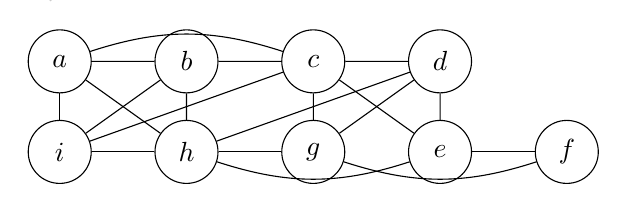
\begin{tikzpicture}[scale=1.15, every node/.style={circle, draw, inner sep=2pt, minimum size=8mm}]
\node (a) at (0,1) {$a$};
\node (b) at (1.4,1) {$b$};
\node (c) at (2.8,1) {$c$};
\node (d) at (4.2,1) {$d$};

\node (i) at (0,0) {$i$};
\node (h) at (1.4,0) {$h$};
\node (g) at (2.8,0) {$g$};
\node (e) at (4.2,0) {$e$};
\node (f) at (5.6,0) {$f$};

\draw (a)--(b)--(c)--(d);
\draw (i)--(h)--(g);
\draw (e)--(f);

\draw (a)--(i);
\draw (b)--(h);
\draw (c)--(g);
\draw (d)--(e);

\draw (a)--(h);
\draw (i)--(b);
\draw (i)--(c);
\draw (h)--(d);
\draw (g)--(d);
\draw (c)--(e);

\draw[bend left=18] (a) to (c);
\draw[bend right=18] (h) to (e);
\draw[bend right=18] (g) to (f);
\end{tikzpicture}
\end{center}

\subsection{Solution}

\subsubsection{Method 1: Euler's criterion}
A connected graph has an Euler circuit if and only if every vertex has even degree.

From the drawing, the degrees are:
\[
\deg(a)=4,\quad \deg(b)=4,\quad \deg(c)=6,\quad \deg(d)=4,\quad \deg(e)=4,
\]
\[
\deg(f)=2,\quad \deg(g)=4,\quad \deg(h)=6,\quad \deg(i)=4.
\]
Every degree is even. The graph is also connected, because each vertex is joined by edges to the rest of the graph.

Therefore, by Euler's criterion, the graph has an Euler circuit. Hence
\[
\boxed{\text{Yes, the graph has an Euler circuit.}}
\]

\subsubsection{Method 2: Exhibit an explicit Euler circuit}
One Euler circuit is
\[
a\to h\to e\to f\to g\to h\to i\to c\to e\to d\to g\to c\to d\to h\to b\to i\to a\to c\to b\to a.
\]
We verify:
\begin{itemize}[leftmargin=*]
  \item it starts and ends at \(a\), so it is a circuit;
  \item every consecutive pair of vertices is joined by an edge in the graph;
  \item each edge of the graph is used exactly once.
\end{itemize}
Hence it is an Euler circuit.

Therefore
\[
\boxed{a\to h\to e\to f\to g\to h\to i\to c\to e\to d\to g\to c\to d\to h\to b\to i\to a\to c\to b\to a}
\]
is an Euler circuit.

\newpage

%====================================================
% QUESTION 5
%====================================================
\section{Question 5 (Can one always add edges to obtain an Euler circuit?)}

\subsection{Problem}
Is it true that by adding edges to a simple graph \(G=(V,E)\) (without introducing multiple edges between any pair of vertices) one can always create a graph that has an Euler circuit? Justify the answer.

\subsection{Solution}

\subsubsection{Method 1: A smallest counterexample}
The statement is \emph{false}.

Take the simple graph \(G=K_2\), the complete graph on two vertices. It has one edge, and both vertices have degree \(1\), so it does not have an Euler circuit.

Because \(K_2\) is already complete on its vertex set, there is no additional edge that can be added without creating a multiple edge. Therefore it is impossible to modify \(K_2\) by adding edges alone so as to obtain an Eulerian graph.

Hence
\[
\boxed{\text{No, this is not always possible.}}
\]

\subsubsection{Method 2: A general family of counterexamples}
More generally, let \(G=K_{2m}\) for any integer \(m\ge 1\). This graph is complete, so no new edges can be added. Every vertex has degree
\[
2m-1,
\]
which is odd. A connected graph can have an Euler circuit only if every vertex has even degree. Therefore \(K_{2m}\) is not Eulerian.

Since no edges can be added to a complete graph, \(K_{2m}\) can never be turned into a graph with an Euler circuit by adding edges only.

Thus
\[
\boxed{\text{The claim is false; complete graphs }K_{2m}\text{ provide counterexamples.}}
\]

\newpage

%====================================================
% QUESTION 6
%====================================================
\section{Question 6 (Ex.\ 10.5.7, 10.5.8: One-stroke drawings)}

\subsection{Problem}
Determine whether each of the pictures shown below can be drawn with a pencil in a continuous motion without lifting the pencil or retracing part of the picture.

\begin{center}
\begin{minipage}{0.35\textwidth}
\centering
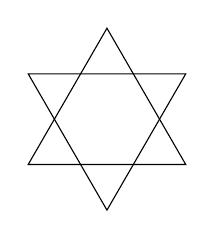
\begin{tikzpicture}[scale=1.0]
\draw (-1,0) -- (1,0) -- (0,-1.73) -- cycle;
\draw (-1,-1.15) -- (1,-1.15) -- (0,0.58) -- cycle;
\end{tikzpicture}
\end{minipage}
\hfill
\begin{minipage}{0.45\textwidth}
\centering
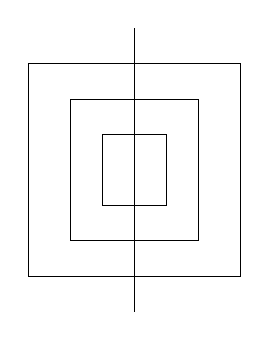
\begin{tikzpicture}[scale=0.9]
\draw (0,0) rectangle (3,3);
\draw (0.6,0.5) rectangle (2.4,2.5);
\draw (1.05,1.0) rectangle (1.95,2.0);
\draw (1.5,-0.5) -- (1.5,3.5);
\end{tikzpicture}
\end{minipage}
\end{center}

\subsection{Solution}

\subsubsection{Method 1: Use the Euler-trail criterion}
A connected graph can be drawn in one continuous stroke without retracing if and only if it has either:
\begin{itemize}[leftmargin=*]
  \item no odd-degree vertices (Euler circuit), or
  \item exactly two odd-degree vertices (Euler trail).
\end{itemize}

\begin{enumerate}[label=(\alph*)]
\item For the six-pointed star, the six outer tips each have degree \(2\), and the six intersection points each have degree \(4\). Thus every vertex has even degree, and the figure is connected. Therefore it has an Euler circuit, so it can be drawn in one stroke.

Hence
\[
\boxed{\text{Yes, the left picture can be drawn in one stroke.}}
\]

\item For the nested-square picture with the vertical line, every intersection of the vertical line with a square contributes degree \(4\). The only odd-degree vertices are the two endpoints of the vertical line, each of degree \(1\). The figure is connected, and it has exactly two odd vertices, so it has an Euler trail (but not an Euler circuit).

Therefore
\[
\boxed{\text{Yes, the right picture can be drawn in one stroke.}}
\]
\end{enumerate}

\newpage
\subsubsection{Method 2: Start-end reasoning}
\begin{enumerate}[label=(\alph*)]
\item In the star figure, every time one enters an intersection or tip, there is a matching unused edge to leave by; no dead end is forced. Since there is no special starting or ending point forced by parity, one may begin at any point and return to the starting point after traversing all edges. So the figure is drawable in one continuous closed stroke.

Thus
\[
\boxed{\text{Yes.}}
\]

\item In the nested-square figure, the only natural starting and ending points are the two ends of the vertical segment, because those are the only places where the drawing has degree \(1\). One can start at the top endpoint, move through all square intersections, and finish at the bottom endpoint without repeating an edge. Thus the figure has an open one-stroke drawing.

Hence
\[
\boxed{\text{Yes, beginning at one endpoint of the vertical line and ending at the other.}}
\]
\end{enumerate}

\newpage

%====================================================
% QUESTION 7
%====================================================
\section{Question 7 (Ex.\ 10.5.16: When do \(K_n\) and \(C_n\) have Euler circuits?)}

\subsection{Problem}
For what values of \(n\) do these graphs have an Euler circuit?
\begin{enumerate}[label=(\alph*)]
\item \(K_n\),
\item \(C_n\).
\end{enumerate}

\subsection{Solution}

\subsubsection{Method 1: Apply Euler's criterion}
A connected graph has an Euler circuit if and only if every vertex has even degree.

\begin{enumerate}[label=(\alph*)]
\item In \(K_n\), each vertex is adjacent to every other vertex, so each vertex has degree
\[
n-1.
\]
Also, \(K_n\) is connected for every \(n\ge 1\). Therefore \(K_n\) has an Euler circuit exactly when
\[
n-1 \text{ is even},
\]
that is, exactly when
\[
n \text{ is odd}.
\]
Hence
\[
\boxed{K_n \text{ has an Euler circuit exactly for odd }n.}
\]

\item In \(C_n\), every vertex has degree \(2\), which is even. The cycle graph \(C_n\) is connected (for the usual definition \(n\ge 3\)). Therefore every cycle graph has an Euler circuit.

Thus
\[
\boxed{C_n \text{ has an Euler circuit for every } n\ge 3.}
\]
\end{enumerate}

\subsubsection{Method 2: Direct structural interpretation}
\begin{enumerate}[label=(\alph*)]
\item In a complete graph \(K_n\), traversing an Euler circuit would require every time the walk enters a vertex to leave along a different unused edge, so the degree at each vertex must be even. Since the degree is \(n-1\), this forces \(n\) to be odd. Conversely, when \(n\) is odd, \(K_n\) is connected and all degrees are even, so an Euler circuit exists.

Therefore
\[
\boxed{K_n \text{ is Eulerian if and only if } n \text{ is odd}.}
\]

\item The graph \(C_n\) is itself a single cycle:
\[
v_1\to v_2\to \cdots \to v_n\to v_1.
\]
This closed walk uses every edge exactly once. Hence \(C_n\) is automatically an Euler circuit for the graph.

So
\[
\boxed{C_n \text{ has an Euler circuit for every } n\ge 3.}
\]
\end{enumerate}

\newpage

%====================================================
% QUESTION 8
%====================================================
\section{Question 8 (Ex.\ 10.5.20, 10.5.21: Hamilton circuits)}

\subsection{Problem}
Determine whether each of the given graphs below has a Hamilton circuit. If it does, find such a circuit. If it does not, give an argument to show why no such circuit exists.

\begin{center}
\begin{minipage}{0.45\textwidth}
\centering
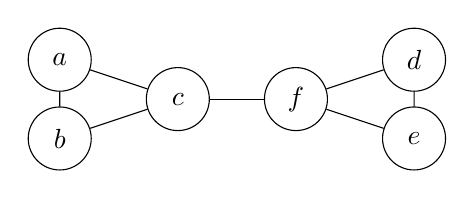
\begin{tikzpicture}[scale=1.0, every node/.style={circle, draw, inner sep=2pt, minimum size=8mm}]
\node (a) at (0,1) {$a$};
\node (b) at (0,0) {$b$};
\node (c) at (1.5,0.5) {$c$};
\node (f) at (3.0,0.5) {$f$};
\node (d) at (4.5,1) {$d$};
\node (e) at (4.5,0) {$e$};

\draw (a)--(b)--(c)--(a);
\draw (c)--(f);
\draw (f)--(d)--(e)--(f);
\end{tikzpicture}
\end{minipage}
\hfill
\begin{minipage}{0.40\textwidth}
\centering
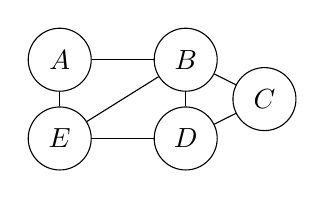
\begin{tikzpicture}[scale=1.0, every node/.style={circle, draw, inner sep=2pt, minimum size=8mm}]
\node (A) at (0,1) {$A$};
\node (E) at (0,0) {$E$};
\node (B) at (1.6,1) {$B$};
\node (D) at (1.6,0) {$D$};
\node (C) at (2.6,0.5) {$C$};

\draw (A)--(B)--(D)--(E)--(A);
\draw (E)--(B);
\draw (B)--(C)--(D);
\end{tikzpicture}
\end{minipage}
\end{center}

\subsection{Solution}

\subsubsection{Method 1: Use bridges and explicit construction}
\begin{enumerate}[label=(\alph*)]
\item The left graph does \emph{not} have a Hamilton circuit.

The edge \(cf\) is a bridge: if it is removed, the graph breaks into two components,
\[
\{a,b,c\}
\qquad\text{and}\qquad
\{d,e,f\}.
\]
A graph containing a Hamilton circuit cannot have a bridge, because every edge on a Hamilton circuit lies on a cycle, and an edge lying on a cycle cannot be a bridge.

Therefore the left graph has no Hamilton circuit. Hence
\[
\boxed{\text{The left graph has no Hamilton circuit.}}
\]

\item The right graph \emph{does} have a Hamilton circuit. One such circuit is
\[
A\to B\to C\to D\to E\to A.
\]
Each consecutive pair is joined by an edge:
\[
AB,\ BC,\ CD,\ DE,\ EA.
\]
This closed walk visits each vertex exactly once before returning to the start.

Therefore
\[
\boxed{A\to B\to C\to D\to E\to A}
\]
is a Hamilton circuit for the right graph.
\end{enumerate}

\subsubsection{Method 2: Forced-edge analysis}
\begin{enumerate}[label=(\alph*)]
\item In the left graph, the vertices \(a,b,d,e\) each have degree \(2\). In any Hamilton circuit, every degree-\(2\) vertex must use both of its incident edges, because the circuit must enter and leave that vertex exactly once.

Thus a Hamilton circuit would have to contain:
\[
ac,\ bc,\ df,\ ef.
\]
That already forces vertex \(c\) to use both \(ca\) and \(cb\), leaving no remaining capacity at \(c\) to use the bridge edge \(cf\). Similarly, vertex \(f\) would be forced to use \(fd\) and \(fe\), leaving no capacity to use \(fc\). But then there would be no way to connect the two triangles in one Hamilton cycle.

Hence the left graph has no Hamilton circuit:
\[
\boxed{\text{No Hamilton circuit exists in the left graph.}}
\]

\item In the right graph, the vertices \(A\) and \(C\) have degree \(2\). Therefore any Hamilton circuit must use both edges incident with \(A\) and both edges incident with \(C\). So the circuit must contain
\[
AB,\ AE,\ BC,\ CD.
\]
Since \(B\) already uses \(AB\) and \(BC\), it can use no other Hamilton-cycle edges. Since \(C\) uses \(BC\) and \(CD\), and \(A\) uses \(AB\) and \(AE\), the only way to close the cycle through all five vertices is to use
\[
DE
\]
and return via
\[
EA.
\]
Thus the Hamilton circuit is forced to be
\[
A\to B\to C\to D\to E\to A.
\]
Therefore
\[
\boxed{A\to B\to C\to D\to E\to A}
\]
is a Hamilton circuit.
\end{enumerate}

\newpage

%====================================================
% QUESTION 9
%====================================================
\section{Question 9 (Edge bounds for a graph with \(k\) connected components)}

\subsection{Problem}
Given a simple graph \(G\) with \(n\) vertices and \(m\) edges. If \(G\) has exactly \(k\) connected components, prove that
\[
n-k \le m \le \frac{(n-k)(n-k+1)}{2}.
\]

\subsection{Solution}

\subsubsection{Method 1: Componentwise bounds}
Let the connected components of \(G\) have vertex counts
\[
n_1,n_2,\dots,n_k,
\]
where each \(n_i\ge 1\) and
\[
n_1+n_2+\cdots+n_k=n.
\]

\paragraph{Lower bound.}
Each connected component on \(n_i\) vertices has at least
\[
n_i-1
\]
edges, because every connected graph contains a spanning tree, and a tree on \(n_i\) vertices has exactly \(n_i-1\) edges. Summing over all components,
\[
m \ge \sum_{i=1}^k (n_i-1)=\sum_{i=1}^k n_i-k=n-k.
\]
So
\[
\boxed{m\ge n-k.}
\]

\paragraph{Upper bound.}
Since the graph is simple, a connected component on \(n_i\) vertices has at most
\[
\binom{n_i}{2}
\]
edges, attained when the component is complete. Therefore
\[
m\le \sum_{i=1}^k \binom{n_i}{2}. \tag{1}
\]

We now maximize the right-hand side under the constraint \(n_1+\cdots+n_k=n\) with \(n_i\ge 1\). The sum is maximized by making one component as large as possible and all others as small as possible. To justify this, suppose \(x\ge y\ge 2\). Then
\begin{align*}
\binom{x+1}{2}+\binom{y-1}{2}-\left(\binom{x}{2}+\binom{y}{2}\right)
&=x-(y-1)\\
&=x-y+1\\
&\ge 1.
\end{align*}
So moving one vertex from a smaller nontrivial component to a larger component increases the total number of edges.

Repeating this process shows that the maximum occurs when
\[
(n_1,n_2,\dots,n_k)=(n-k+1,1,1,\dots,1).
\]
Then \((1)\) gives
\[
m\le \binom{n-k+1}{2}
=\frac{(n-k)(n-k+1)}{2}.
\]
Hence
\[
\boxed{m\le \frac{(n-k)(n-k+1)}{2}.}
\]

Combining the two bounds,
\[
\boxed{n-k \le m \le \frac{(n-k)(n-k+1)}{2}.}
\]

\subsubsection{Method 2: Spanning forest for the lower bound, and a quadratic inequality for the upper bound}
Again let the component sizes be \(n_1,\dots,n_k\), with
\[
n_i\ge 1,\qquad \sum_{i=1}^k n_i=n.
\]

\paragraph{Lower bound via spanning forest.}
Choose a spanning tree in each connected component. The union of these trees is a spanning forest of \(G\). A spanning tree in the \(i\)th component uses \(n_i-1\) edges, so the spanning forest uses
\[
\sum_{i=1}^k (n_i-1)=n-k
\]
edges. Since this forest is a subgraph of \(G\), the graph \(G\) has at least that many edges:
\[
\boxed{m\ge n-k.}
\]

\paragraph{Upper bound via \(x_i=n_i-1\).}
Set
\[
x_i=n_i-1\qquad (i=1,\dots,k).
\]
Then each \(x_i\ge 0\), and
\[
x_1+x_2+\cdots+x_k=n-k.
\]
Now
\[
\binom{n_i}{2}=\binom{x_i+1}{2}=\frac{x_i(x_i+1)}{2}.
\]
Hence
\[
m\le \sum_{i=1}^k \binom{n_i}{2}
=\frac12\sum_{i=1}^k \bigl(x_i^2+x_i\bigr)
=\frac12\left(\sum_{i=1}^k x_i^2+\sum_{i=1}^k x_i\right).
\]
Because the \(x_i\) are nonnegative,
\[
\sum_{i=1}^k x_i^2 \le \left(\sum_{i=1}^k x_i\right)^2.
\]
Therefore
\begin{align*}
m
&\le \frac12\left(\left(\sum_{i=1}^k x_i\right)^2+\sum_{i=1}^k x_i\right)\\
&=\frac12\bigl((n-k)^2+(n-k)\bigr)\\
&=\frac{(n-k)(n-k+1)}{2}.
\end{align*}
So
\[
\boxed{m\le \frac{(n-k)(n-k+1)}{2}.}
\]

Combining the lower and upper estimates gives
\[
\boxed{n-k \le m \le \frac{(n-k)(n-k+1)}{2}.}
\]

\end{document}